\documentclass[a4paper, 12pt]{article}
\usepackage{amsmath, amssymb, amsfonts, amsthm, mathtools}
\usepackage[utf8x]{inputenc}
\usepackage[T2A]{fontenc} 
\usepackage[russian]{babel}
\usepackage{cmap} 
\usepackage{gensymb}
\usepackage[unicode]{hyperref}
\usepackage{textcomp}
\usepackage{hyperref}
\usepackage{moreverb}
\usepackage{multirow}

\usepackage{graphicx}

\usepackage[margin=1in]{geometry}

\usepackage{fancyhdr}

\newcommand{\bbR}{\mathbb R}
\newcommand{\eps}{\varepsilon}
\newcommand{\bbN}{\mathbb N}
\newcommand{\dif}{\mathrm{d}}
\newcommand{\vsp}{\vspace{\baselineskip}}

\pagestyle{fancy}
\makeatletter
\fancyhead[L]{\footnotesize Оптика}
\fancyhead[R]{\footnotesize ФМХФ МФТИ}
%\fancyfoot[L]{\footnotesize \@author}
\fancyfoot[R]{\thepage}
\fancyfoot[C]{}

\renewcommand{\maketitle}{%
	\noindent{\bfseries\scshape\large\@title\ \mdseries\upshape}\par
	\noindent {\large\itshape\@author}
	\vskip 2ex}
\makeatother

\setlength{\parindent}{0pt}

\title{4.3.5 \\ Саморепродукция}
\author{Егор Берсенев} 
\date{9 февраля 2017 г.}

\begin{document}
	
	\maketitle
	
	\section{Цель работы:} 
	Изучение явления саморепродукции и применение его к измерению параметров периодических структур.

	\section{Оборудование} 
	Лазер, кассета с сетками, мира, короткофокусная линза с микрометрическим винтом, экран, линейка.
	
	\section{Теоретическое введение}
	
	Выражение для плоской монохроматической волны имеет вид 
	\begin{equation}\label{eq:wave}
		E(\mathbf{r}, t) = a_0e^{-i(\omega t - \mathbf{kr} - \psi_0)}, 
	\end{equation}
	где $a_0$ - амплитуда, $\omega$ - круговая частота, $\mathbf{k} = (u, v, q)$ - волновой вектор , $\psi_0$ - начальная фаза. Колебания происходят синфазно во всех точках плоскости:
	\begin{equation}\label{eq:kr}
		\mathbf{kr} = ux + vy + \sqrt{k^2 - u^2 - v^2}\cdot z = const.
	\end{equation}
	
	Для плоской волны \eqref{eq:wave} комплексную амплитуду можно представить в виде
	\begin{equation}\label{eq:to_z}
		f(x, y, z) = a_oe^{i\psi_0}e^{ux+vy}e^{\sqrt{k^2 - u^2 - v^2}\cdot z} = f(x, y, 0)e^{\sqrt{k^2 - u^2 - v^2}\cdot z}.
	\end{equation}
	
	Пусть плоская волна падает нормально на транспарант, расположенный в плоскости $z = 0$. Комплексную амплитуду волны в плоскости $z = 0_+$ получаем, умножив комплексную амплитуду на входе в транспарант на функцию пропускания транспаранта $t(x, y)$. Для простоты далее будем рассматривать случай $t(x, y) = t(x)$. Если функция пропускания периодична с пространственным периодом $d$, то комплексная амплитуда на выходе также будет периодической функцией с периодом $d$
	\begin{equation}\label{eq:decomp}
		f(x, 0_+) = \sum\limits_{-\infty}^{+\infty} c_ne^{iu_nx} = \sum\limits_{-\infty}^{+\infty} c_ne^{i\frac{2\pi}{d}nx},
	\end{equation}
	где коэффициенты $c_n$ можно найти с помощью формулы
	\begin{equation}\label{eq:coeff}
		c_n = \frac{1}{d} \int\limits_{-d/2}^{d/2} f(x, 0_+)e^{-i\frac{2\pi}{d}nx}
	\end{equation}
	
	Для нахождения комплексной амплитуды волны в произвольной плоскости $z = const$ нужно домножить комплексные амплитуды плоских волн в суперпозиции \eqref{eq:decomp} на соответствующий фазовый множитель (равенство \eqref{eq:kr}):
	\begin{equation}\label{eq:to_zz}
		f(x, z) = \sum\limits_{-\infty}^{+\infty} c_ne^{iu_nx}e^{\sqrt{k^2 - u_n^2}\cdot z}
	\end{equation}
	То есть, каждая плоская волна приобретает дополнительный набег фаз $\varphi_n$. Для параксиальных волн $(u_n \ll 1)$
	\begin{equation}\label{eq:parax}
		\varphi_n = \sqrt{k^2 - u_n^2}\cdot z \approx kz - \frac{u_n^2}{2k}z
	\end{equation}
	Таким образом, для любых двух плоских волн разность набегов фазы равна
	\begin{equation}\label{eq:phase}
		\Delta\varphi_{n, m} = (u_m^2 - u_n^2)\frac{z}{2k} = (m^2 - n^2)\frac{\pi\lambda}{d^2}z.
	\end{equation}
	
	В плоскости
	\begin{equation}\label{eq:end_formula}
		z_N = \frac{2d^2}{\lambda}N
	\end{equation}
	разница набегов фаз становится кратной $2\pi$. Поэтому в результате интерференции волн в этой плоскости получается изображение, тождественное исходному периодическому объекту. Это и есть \textit{эффект саморепродукции}.
	
	\section{Эксперимент}
	
	\begin{figure}[h!]\label{fig:scheme}
		\begin{center}
			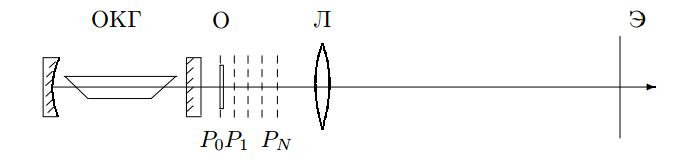
\includegraphics[scale=0.8]{scheme}
			\caption{Схема экспериментальной установки}
		\end{center}
	\end{figure}

	В нашем эксперименте $\lambda = 532\,\text{нм}$.
	
	\subsection{Исследование двумерных решеток}
	
	\subsubsection{Исследование по пространственному спектру}
	
	\begin{table}[h!]\label{tab:net_spectre}
		\centering
		\caption{Исследование с помощью спектра. $L = 133cm$.}
		\begin{tabular}{|c|c|c|c|c|c|c|}
			\hline
			net number & 1    & 2    & 3    & 4    & 5    & 6   \\ \hline
			$l$, cm      & 0.42 & 0.63 & 0.90 & 1.40 & 1.85 & 3.6 \\ \hline
		\end{tabular}
	\end{table}

	 По формуле $ d = \frac{L\lambda}{l} $ определим период решетки $d$
	 
	 \subsubsection{Исследование по увеличенному изображению}
	 
	 
	 \begin{table}[h!]\label{tab:ampl_img}
	 	\centering
	 	\caption{Исследование по изображению. $a = 5.5cm$, $b = 127cm$.}
	 	\begin{tabular}{|c|c|c|c|c|}
	 		\hline
	 		net number & 1    & 2    & 3    & 4    \\ \hline
	 		p, cm      & 0.43 & 0.25 & 0.19 & 0.13 \\ \hline
	 	\end{tabular}
	 \end{table}
	
	По формуле $d = \frac{a}{b}p$ определим период решетки $d$.
	
	\vspace{4\baselineskip}
	
	\subsubsection{Исследование репродукции}
	
	\begin{table}[h!]\label{tab:reproduct}
		\centering
		\caption{Исследование репродукции}
		\begin{tabular}{|c|c|c|c|c|c|}
			\hline
			\multicolumn{2}{|c|}{periodic net 1}         & \multicolumn{2}{c|}{periodic net 2} & \multicolumn{2}{c|}{periodic net 3} \\ \hline
			N               & $z_N$, cm              & N           & $z_N$, cm         & N           & $z_N$, cm         \\ \hline
			-2              & 73,2                  & -5          & 78,9             & -4          & 73,9             \\ \hline
			-1              & 68,2                  & -4          & 75,5             & -3          & 70               \\ \hline
			0               & 61,7                  & -3          & 72               & -2          & 67,3             \\ \hline
			1               & 55,2                  & -2          & 68,9             & -1          & 64,9             \\ \hline
			2               & 50                    & -1          & 65,1             & 0           & 61,7             \\ \hline
			\multicolumn{2}{|c|}{\multirow{5}{*}{}} & 0           & 61,7             & 1           & 59,3             \\ \cline{3-6} 
			\multicolumn{2}{|c|}{}                  & 1           & 57,3             & 2           & 56,5             \\ \cline{3-6} 
			\multicolumn{2}{|c|}{}                  & 2           & 53,3             & 3           & 51,9             \\ \cline{3-6} 
			\multicolumn{2}{|c|}{}                  & 3           & 50,7             & 4           & 49,4             \\ \cline{3-6} 
			\multicolumn{2}{|c|}{}                  & 4           & 47,4             & \multicolumn{2}{c|}{}          \\ \hline
		\end{tabular}
	\end{table}

	\begin{figure}[h!]
		\begin{center}
			\begin{minipage}{0.49\textwidth}
				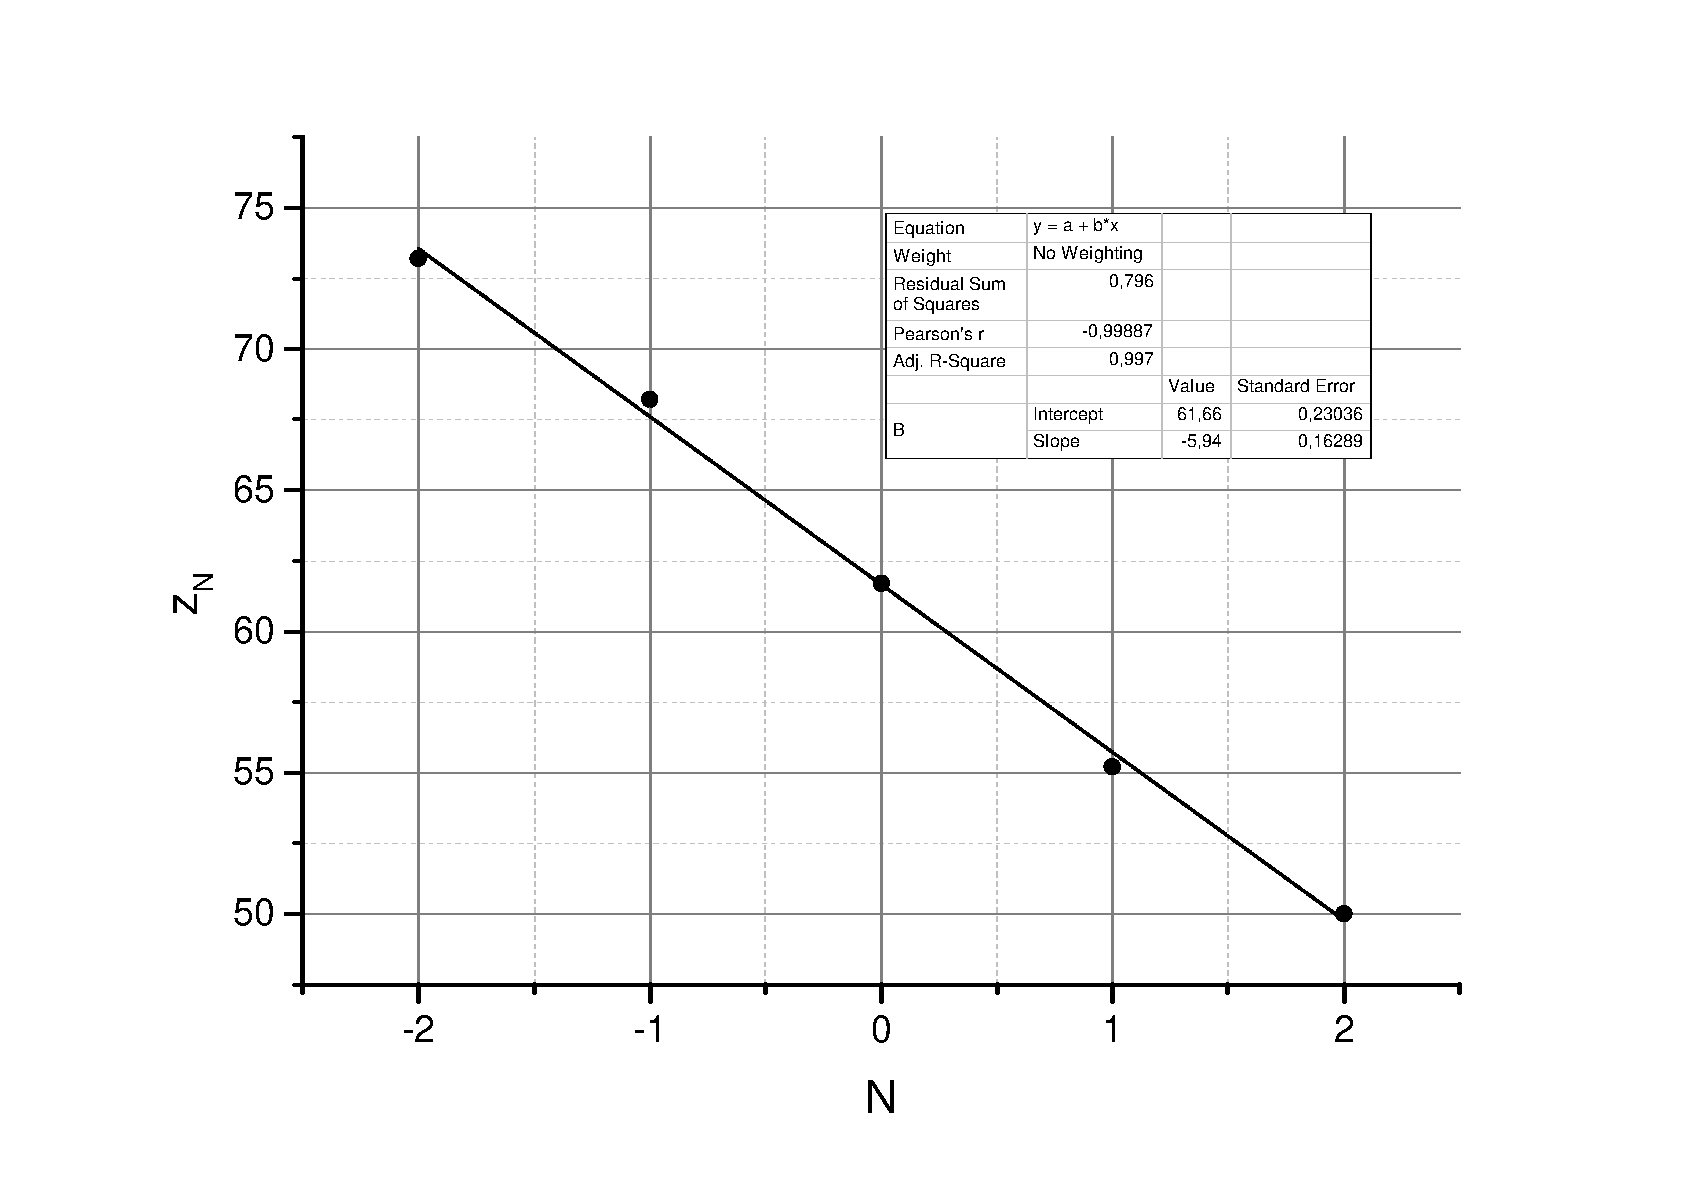
\includegraphics[width=\textwidth]{net_1}
				\caption{Сетка №1}
			\end{minipage}
			\hfill
			\begin{minipage}{0.49\textwidth}
				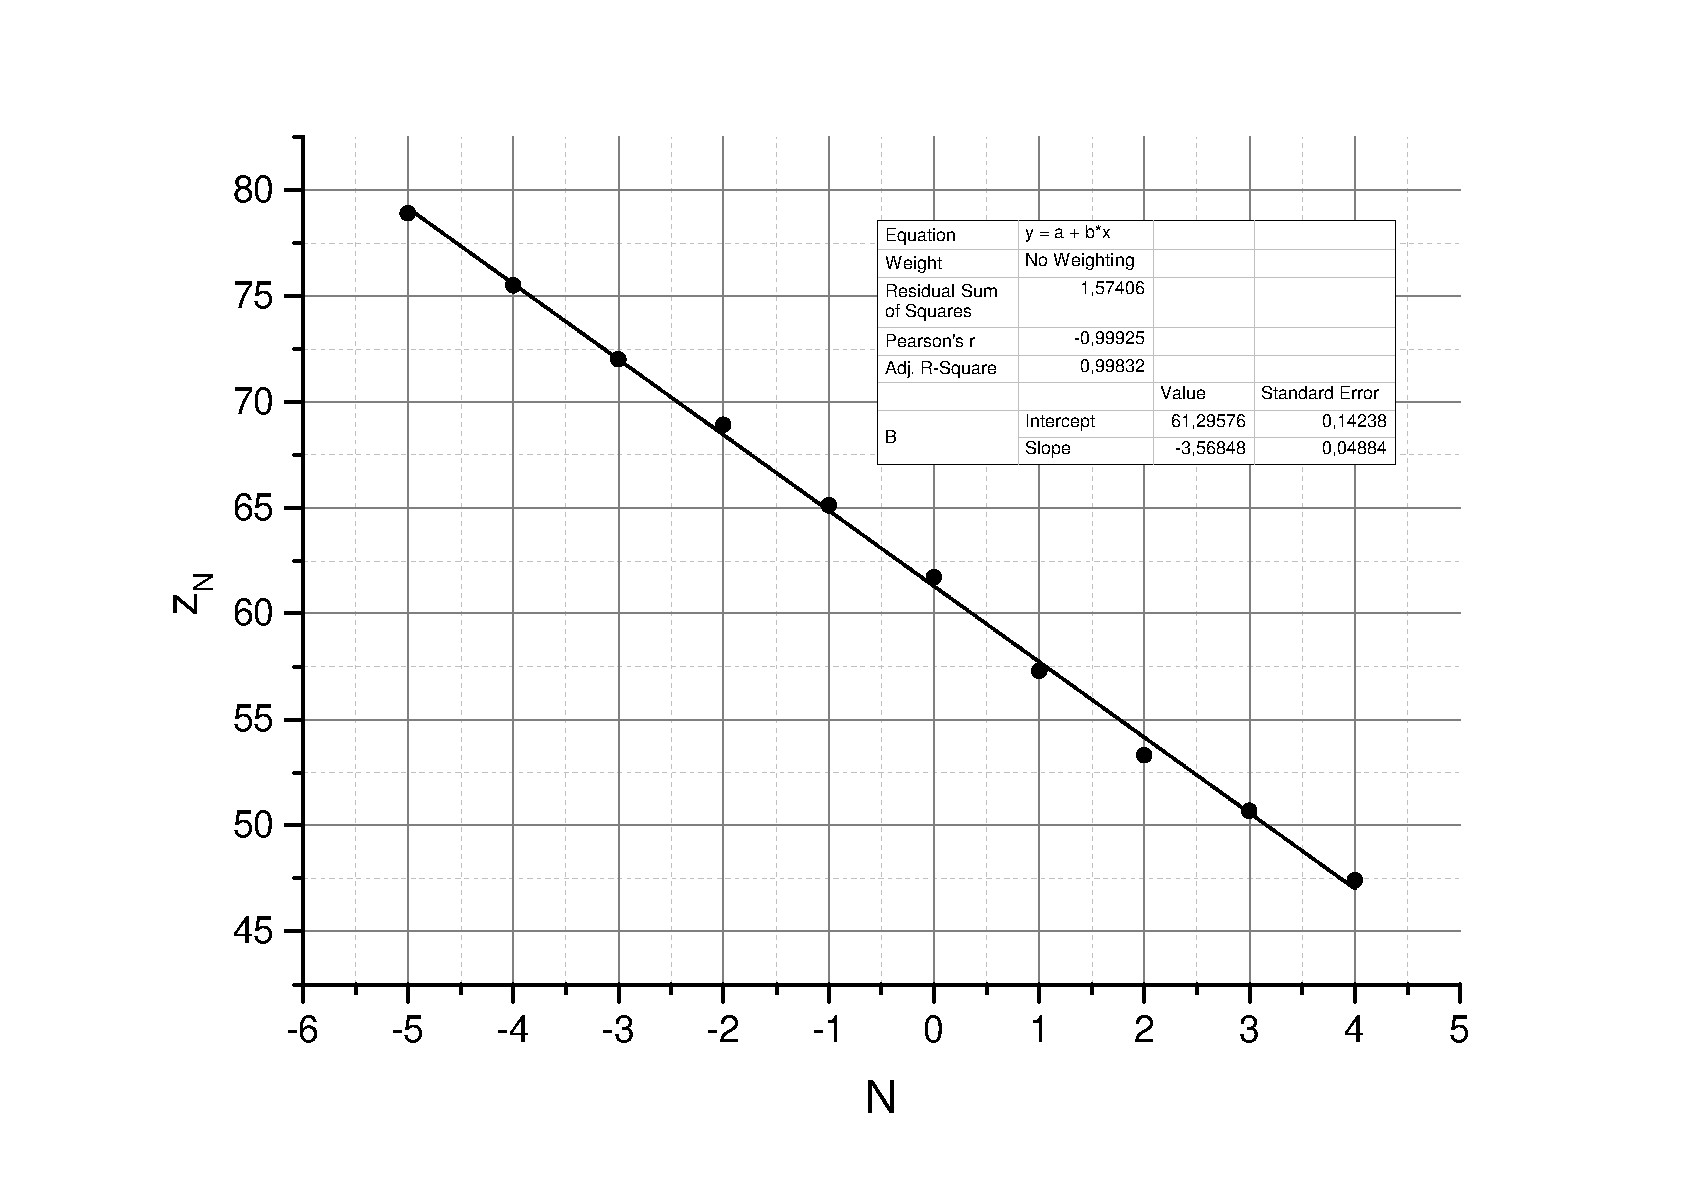
\includegraphics[width=\textwidth]{net_2}
				\caption{Сетка №2}
			\end{minipage}
			\\
			\begin{minipage}{0.49\textwidth}
				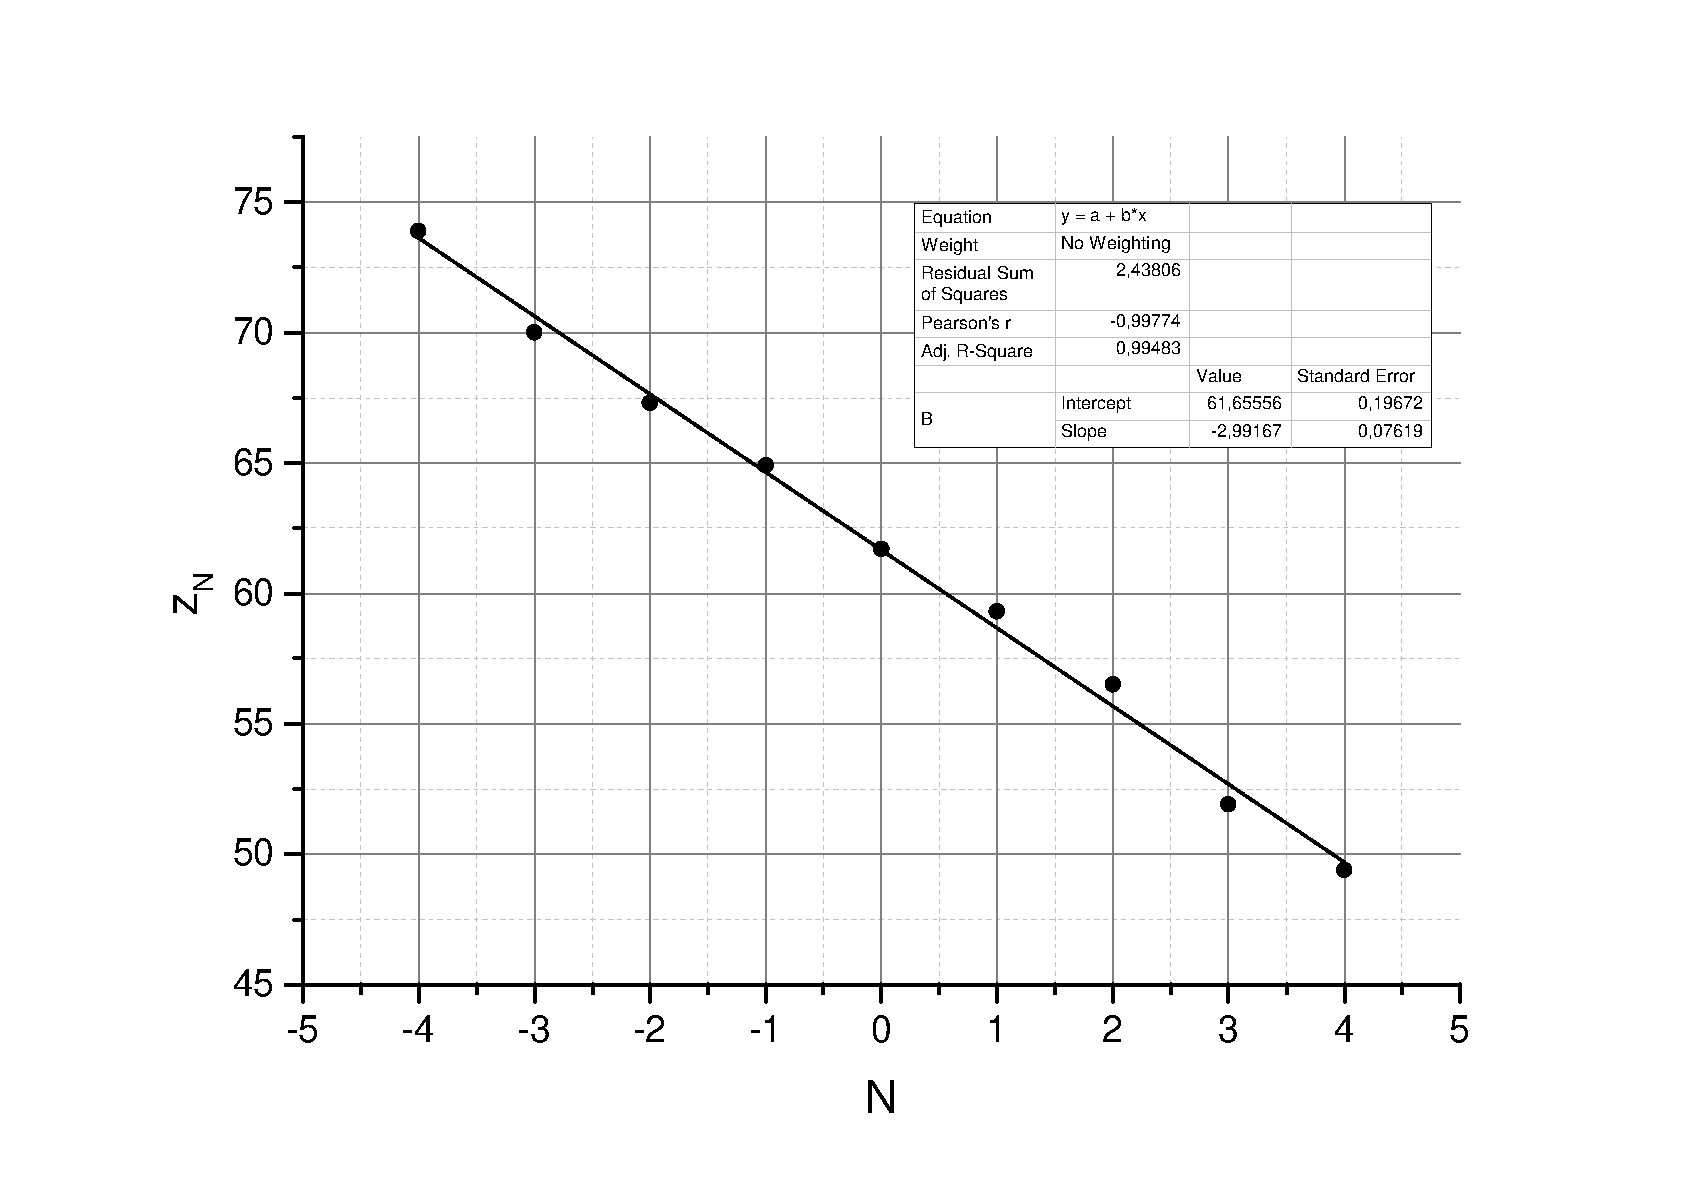
\includegraphics[width=\textwidth]{net_3}
				\caption{Сетка №3}
			\end{minipage}
		\end{center}
	\end{figure}		
	
	По графикам найдем углы наклона прямых и по формуле \eqref{eq:end_formula} определим период решеток $d$.
	
	\subsection{Исследование решеток миры}
	
	\begin{table}[h!]\label{tab:miras}
		\centering
		\caption{Исследование решеток миры}
		\begin{tabular}{|c|c|c|c|}
			\hline
			\multicolumn{2}{|c|}{по спектру} & \multicolumn{2}{c|}{по изображению} \\ \hline
			мира 25        & мира 20         & мира 25          & мира 20          \\ \hline
			l = 1.8        & l = 1.35        & p = 0.1          & p = 0.14         \\ \hline
		\end{tabular}
	\end{table}
	
	\begin{table}[h!]\label{tab:repr_miras}
		\centering
		\caption{Репродукция на решетках миры}
		\begin{tabular}{|c|c|c|c|c|c|c|c|c|c|c|}
			\hline
			\multicolumn{11}{|l|}{мира 25}                                                                    \\ \hline
			N    & -4   & -3 & -2 & -1   & 0    & 1    & 2    & 3    & 4                  & 5                 \\ \hline
			$z_N$ & 75   & 72 & 69 & 66   & 64,1 & 61   & 58   & 55   & 52                 & 49                \\ \hline
			\multicolumn{11}{|l|}{мира 20}                                                                    \\ \hline
			N    & -3   & -2 & -1 & 0    & 1    & 2    & 3    & 4    & \multicolumn{2}{c|}{\multirow{2}{*}{}} \\ \cline{1-9}
			$z_N$ & 79,5 & 74 & 69 & 64,1 & 59   & 53,9 & 48,1 & 43,2 & \multicolumn{2}{c|}{}                  \\ \hline
		\end{tabular}
	\end{table}

	\begin{figure}[h!]
		\begin{center}
			\begin{minipage}{0.49\textwidth}
				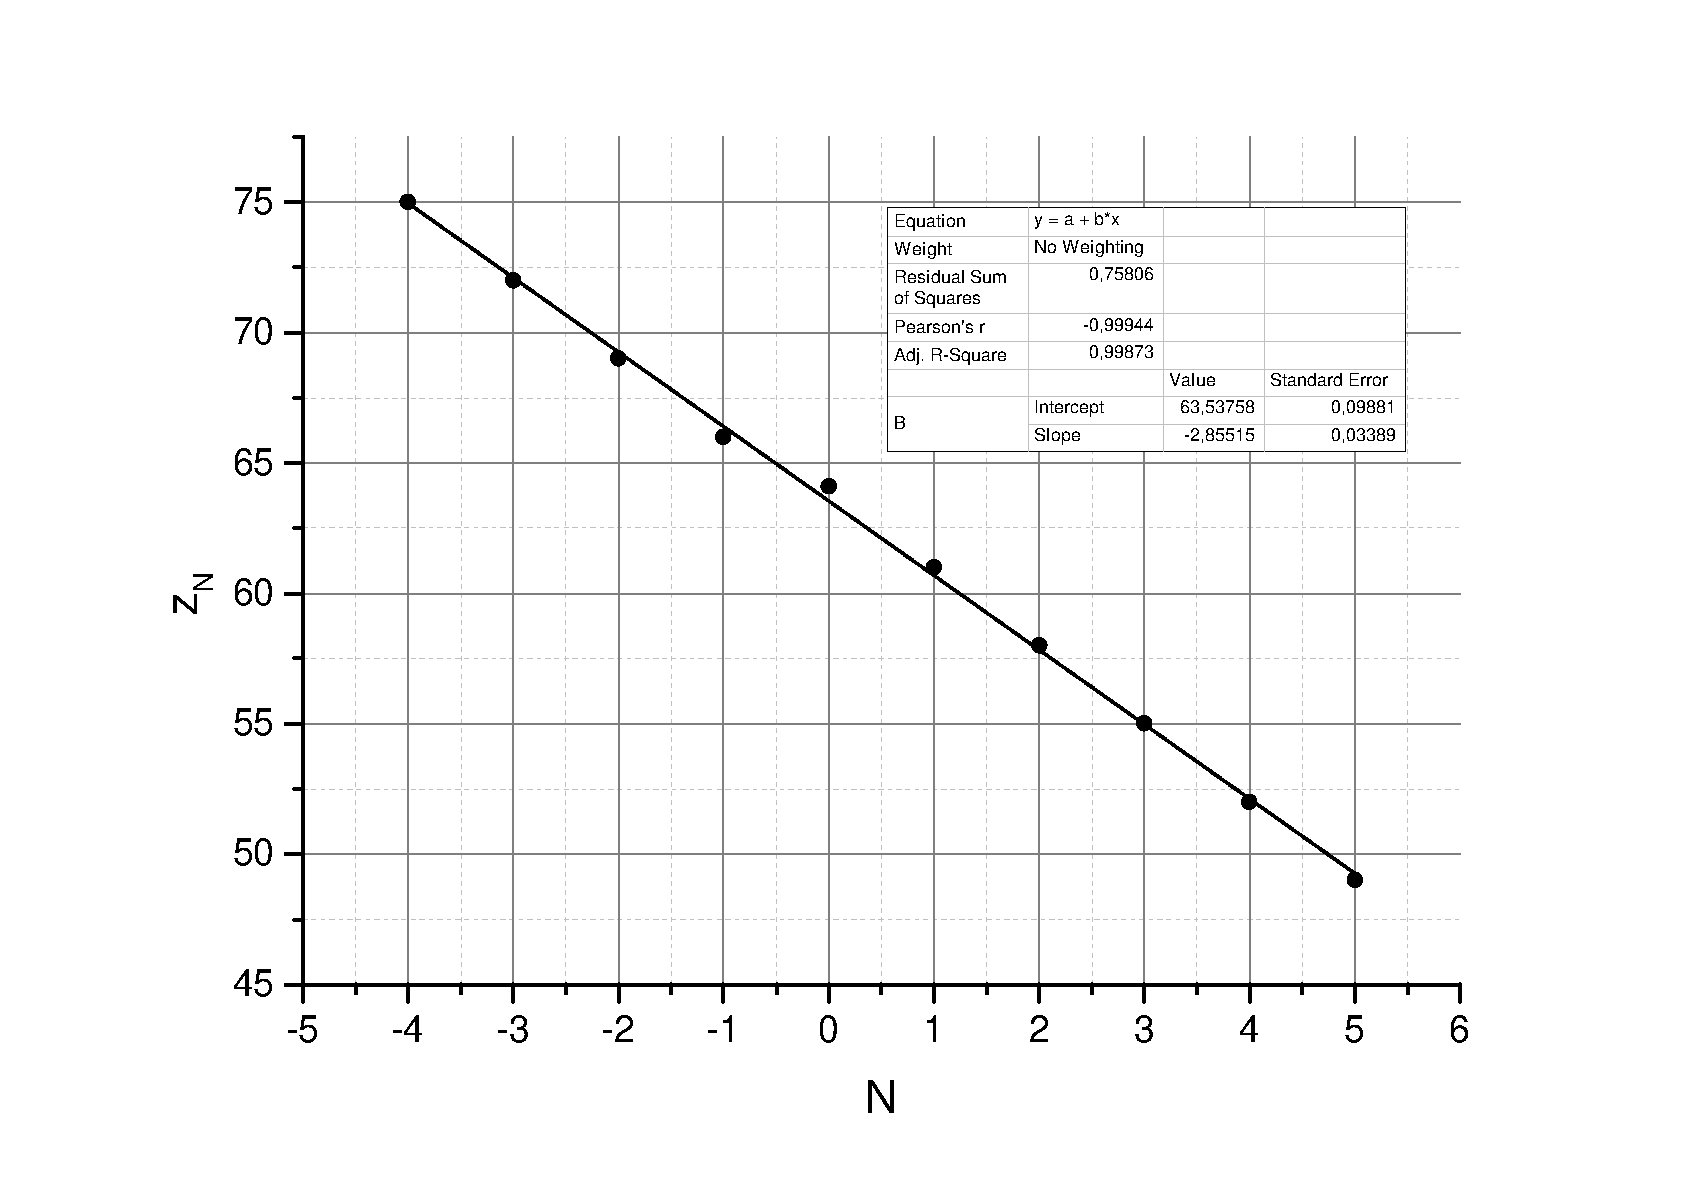
\includegraphics[width=\textwidth]{mira_25}
				\caption{мира 25}
			\end{minipage}
			\hfill
			\begin{minipage}{0.49\textwidth}
				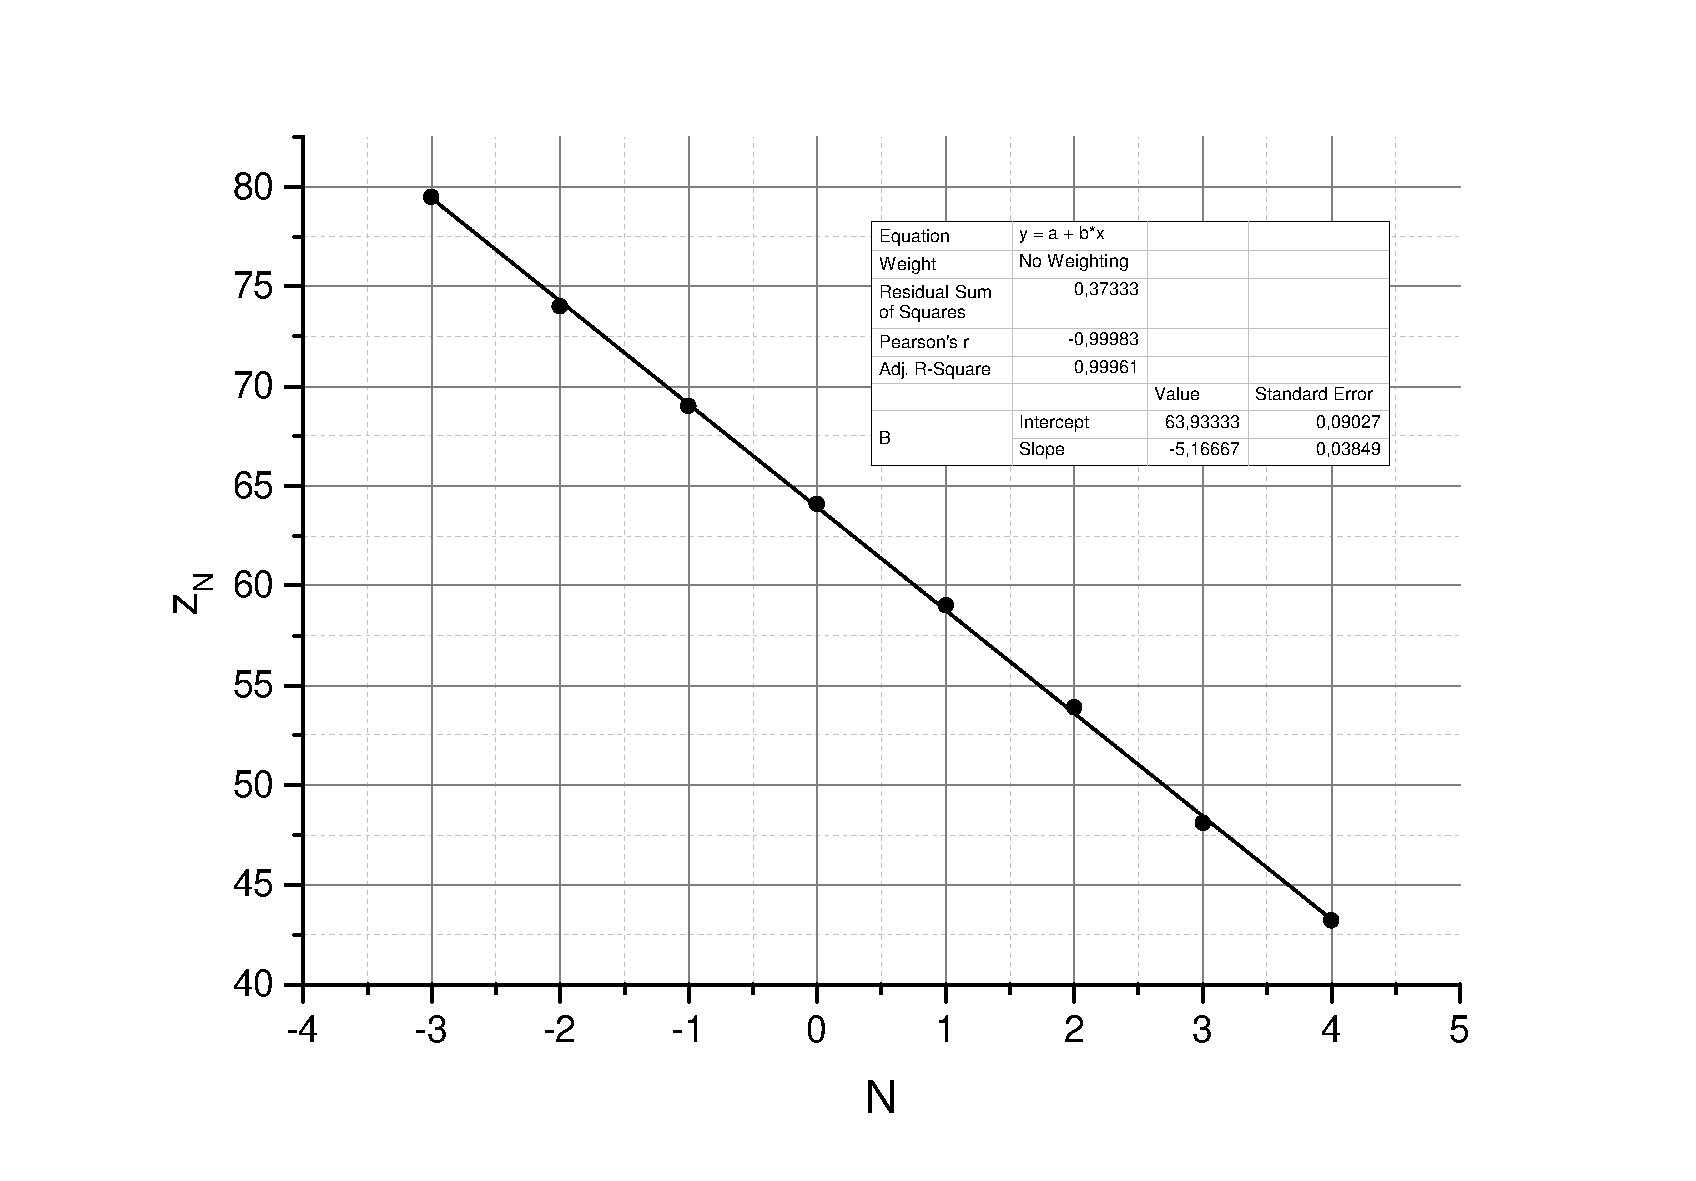
\includegraphics[width=\textwidth]{mira_20}
				\caption{мира 20}
			\end{minipage}
		\end{center}
	\end{figure}
	
	Для решеток миры проведем расчеты, аналогичные расчетам для сеток.
	
	\section{Результаты}
	Сведем все результаты в одну таблицу.
	
	\begin{table}[h!]\label{tab:mira_res}
		\centering
		\caption{Периоды решеток миры в микрометрах}
		\begin{tabular}{|c|c|c|c|}
			\hline
			& spectre      & amplified image & reproduction  \\ \hline
			мира 25 & $39.8\pm4.8$ & $42.63\pm5.5$   & $43.57\pm8.7$ \\ \hline
			мира 20 & $53.0\pm6.4$ & $58.1\pm7.6$    & $58.6\pm11.7$ \\ \hline
		\end{tabular}
	\end{table}
	
	\vspace{4\baselineskip}
	
	\begin{table}[h!]\label{tab:net_res}
		\centering
		\caption{Результаты для сеток}
		\begin{tabular}{|c|c|c|c|c|l|c|}
			\hline
			\multicolumn{7}{|c|}{spectre}                                                                                                    \\ \hline
			net number   & 1              & 2              & 3             & 4            & \multicolumn{1}{c|}{5}            & 6            \\ \hline
			$d$, $\mu m$ & $169.8\pm20.4$ & $113.2\pm13.6$ & $78.6\pm9.4$  & $50.5\pm6.1$ & \multicolumn{1}{c|}{$38.2\pm4.6$} & $19.7\pm2.4$ \\ \hline
			\multicolumn{7}{|c|}{amplified image}                                                                                            \\ \hline
			net number   & 1              & 2              & 3             & 4            & \multicolumn{2}{l|}{\multirow{2}{*}{}}           \\ \cline{1-5}
			$d$, $\mu m$ & $187.7\pm24.4$ & $108.3\pm14.1$ & $84.3\pm11.0$ & $54.7\pm7.1$ & \multicolumn{2}{l|}{}                            \\ \hline
			\multicolumn{7}{|c|}{reproduction}                                                                                               \\ \hline
			net number   & 1              & 2              & 3             & \multicolumn{3}{c|}{\multirow{2}{*}{}}                          \\ \cline{1-4}
			$d$, $\mu m$ & $125.7\pm25.1$ & $97.4\pm19.5$  & $89.2\pm17.8$ & \multicolumn{3}{c|}{}                                           \\ \hline
		\end{tabular}
	\end{table}
	
	\section{Вывод}
	
	В проделанной работе было изучено явление саморепродукции изображения периодической структуры при освещении монохроматическим светом. Также были изучены методы определения параметров периодических структур и получены их значения.
	
	
\end{document}